\section{Shared parameter server}
\label{ivl-sec:shared-parameter-server}

Algorithms such as SGD require updating parameters by either adding
or subtracting. The adder object only supports addition. If we would try subtracting
then the previous bounds calculated do not hold with negative values. Executing
Algorithm~\ref{ivl-alg:ivl-adder} with negative values can cause a read to return a value
that is outside the bounds. Figure~\ref{ivl-img:negative-values} depicts an execution in which $p_3$ returns $-1$,
although the return value is bounded by $0$ and $1$. $p_3$ reads $v[1]$ before $p_1$
adds $1$. $p_1$ and $p_2$ both complete their {\sc update} operations, and then $p_3$
reads $v[2]$. Thus the {\sc read} executed by $p_3$ returns a $-1$.

\begin{figure}[b]
    \centering
    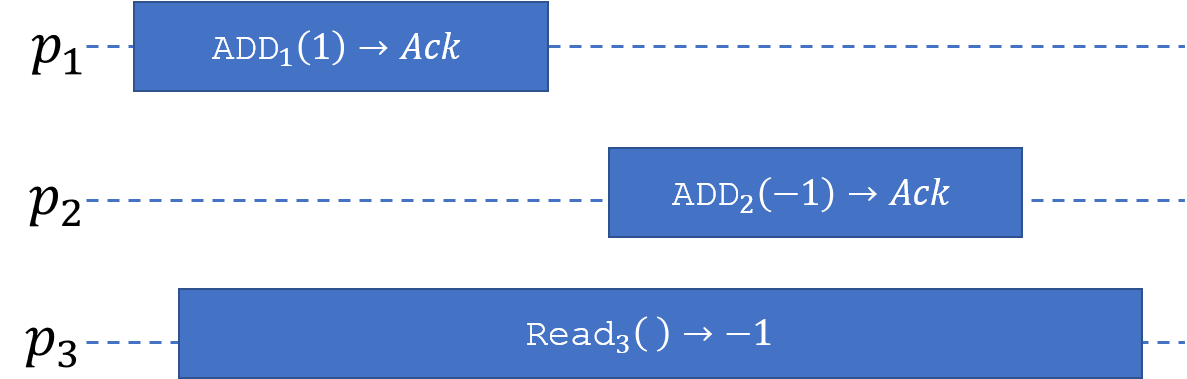
\includegraphics[width=0.5\textwidth]{images/negativeValues.png}
    \caption{A concurrent history for an adder object with four processes. $p_1$ and
    $p_2$ add $1$ and $-1$ respectively, while $p_3$ reads. $p_3$ reads $v[1]$
    before $p_1$ writes, thereby reading $0$, followed by $p_1$ and $p_2$ finishing their writes.
    Finally $p_3$ completes its read, returning $-1$.}
    \label{ivl-img:negative-values}
\end{figure}

We define a \emph{parameter} object, which supports operations {\sc update}($v$) such that $v \in \mathds{R}$ and
{\sc read}(). In a similar fashion to the adder object, the sequential specification
of the parameter object is that the read returns the sum of all the values passed to
the {\sc update} operations that precede it, and $0$ if no such operation exists.

\begin{algorithm}
    \begin{algorithmic}
        \State shared adder $a_p, a_n$ \Comment{Shared adders for positive and negative numebrs}
        \Statex
        \Procedure{update$_i$}{$v$}
        \If{$v \geq 0$}
        \State $a_p$.{\sc update}$_i$($v$)
        \Else
        \State $a_n$.{\sc update}$_i$($-1 \cdot v$)
        \EndIf
        \EndProcedure
        \Statex
        \Procedure{read}{}
        \State $v_1 \gets a_p$.{\sc read}()
        \State $v_2 \gets a_n$.{\sc read}()
        \State $v_3 \gets a_p$.{\sc read}()
        \State $v_4 \gets a_n$.{\sc read}()
        \State \textbf{return} $\max \{v_1, v_3\} - \max \{v_2, v_4\}$
        \EndProcedure
    \end{algorithmic}
    \caption{Algorithm for IVL parameter object.}
    \label{ivl-alg:ivl-parameter}
\end{algorithm}

We implement this object using two IVL adders, $a_p$ and $a_n$. When a process wishes to
update with a positive value, it does so by adding to $a_p$, otherwise, it adds the value to $a_n$.
This implementation is wait-free and built from SWMR registers only,
with a step complexity of $O(1)$ for {\sc update} operations and $O(n)$
for {\sc read} operations. Algorithm~\ref{ivl-alg:ivl-parameter} presents our implementation of an IVL parameter object.


Furthermore, we show that as both adders are IVL, this implementation is IVL:
\begin{lemma}
    Let $a_1,a_2,\dots, a_k$ be $k$ IVL adder objects. Let $a=\sum_{i=1}^k \alpha_i \cdot a_i$ be a linear
    combination of the $k$ adders. Then object $a$ is also IVL.
    \label{ivl-lmma:combination}
\end{lemma}
\begin{proof}
    Let $a_1, \dots, a_k$ and $\alpha_1, \dots, \alpha_k$ be as defined in the lemma.
    Consider some adder $j$. As it is IVL, there exist two values $v_j^1, v_j^2$ such if
    the read returns $v_j$, such that $v_j^1 \leq v_j \leq v_j^2$. Consider $\alpha_j \cdot v_j$.
    If $\alpha_j > 0$, then $\alpha_j \cdot v_j^1 \leq \alpha_j \cdot  v_j \leq \alpha_j \cdot v_j^2$,
    otherwise the inequality flips, and we get $\alpha_j \cdot v_j^2 \leq \alpha_j \cdot  v_j \leq \alpha_j \cdot v_j^1$.
    Either way, there exist $v_j^{1'}, v_j^{2'}$ such that $v_j^{1'} \leq \alpha_j \cdot  v_j \leq v_j^{2'}$.

    Consider $v = \sum_{i=1}^k \alpha_i \cdot v_i$ as read by $a$. Then:
    \begin{equation}
        \sum_{i=1}^k v_i^{1'} \leq v \leq \sum_{i=1}^k v_i^{2'}
    \end{equation}

    Furthermore, when replacing the read values with the appropriate bounds the histories of $a_1, \dots, a_k$ are linearizable.
    Therefore by composing them we get a linearizable object~\cite{herlihy1990linearizability}. Therefore the linear
    combination of IVL adder objects gives an IVL object.
\end{proof}

With Lemma~\ref{ivl-lmma:combination}, we have shown the following theorem:
\begin{theorem}
    There exists a wait-free IVL implementation of a parameter object using only SWMR registers,
    such that the step complexity of {\sc update} is $O(1)$
    and the step complexity of {\sc read} is $O(n)$.
\end{theorem}

The lower bound proved in Section~\ref{ivl-sec:lower-bound} holds here too, as the reduction can be
done using an update object instead of an adder object, and the proof remains the same. Therefore,
we get the following theorem:
\begin{theorem}
    For any linearizable wait-free implementation of an parameter object with $n$ processes from SWMR registers, the step-complexity
    of the {\sc update} operation is $\Omega(n)$.
    \label{ivl-thm:lower-bound}
\end{theorem}